\IEEEraisesectionheading{\section{简介}
\label{sec:introduction}}

纹理在日常生活中无处不在,它们对于区分图像的不同部分非常重要。纹理是由于物体表面的物理属性的多样性而造成的,物理属性不同表示某个特定表面特征的灰度或者颜色信息不同,不同的物理表面会产生不同的纹理图像,例如布纹、草地、砖砌地面的等。然而,对于自然纹理图像而言这种重复模式往往是近似的和复杂的,难以用语言描述,而人类对纹理的感受多是与心理效果相结合的,因此,对纹理很难下一个确切的定义,但它对于描述图像非常有用。

一般而言,纹理图像中的灰度分布具有某种周期性,即使灰度变化是随机的,它也具有一定的统计特性。J.K.Hawkins 对纹理给出了一个比较详细的描述,他认为纹理有三个主要的标志:1)某种局部的序列性在比该序列更大的区域内不断重复;2)序列是由基本元素非随机排列组成的;3)各部分大致是均匀的统一体,在纹理区域内的任何地方都有大致相同的结构尺寸。当然,这些也只是从感觉上看来是合理的,并不能的出定量的纹理测度。正因如此,对纹理特征的研究方法也是各种各样的。

作为提取信息的一种手段,纹理分析使用各种数学方法来表征图像中灰度分布的变化。纹理分析有主要两种不同的方式:统计方法和句法结构方法。纹理分析的一个重要技术是构建图像的特征,这些特征通常以特征向量的形式表示,这些特征向量可以用于与纹理相关的下游任务,如纹理分割等。 

纹理分割是图像处理中的一个重要问题,旨在对具有相同纹理的区域进行识别和划分。在某一区域内,图像的纹理是一致的,即该区域的一些统计量在某种程度上是恒定的或周期性的。首先通过对图像进行纹理分析来构建一组特征向量,然后根据是否有各种纹理的先验知识,以有监督或无监督的方式对其分类,最终将图像分割为不同的区域。如图 \ref{fig:texture_seg} 所示,原始图像可以看作由两种不同的纹理所构成,两种纹理近似分布于一个圆形的内部和外部,在图像进行纹理分析和纹理分割后,图像被按照纹理边界划分为两个区域,同一区域内的纹理是相同的周期性的。

\begin{figure}[!t]
  \vspace{-0.3cm}
  \centering
  \centerline{
  \begin{minipage}[b]{\linewidth} 
  \subfloat[]{
    \begin{minipage}[b]{0.45\linewidth} 
      \centering
      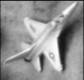
\includegraphics[width=\linewidth]{fig1_a}
     \end{minipage}
  }
  \hfill
    \subfloat[]{
    \begin{minipage}[b]{0.45\linewidth}
      \centering
      
\includegraphics[width=\linewidth]{fig1_b}
       \end{minipage}
  }
  \end{minipage}}
  \caption{合成纹理图像及其基准分割图像示例:(a) 合成纹理图像, (b) 基准分割图像.}
  \label{fig:texture_seg}
  \vspace{-0.5cm}
\end{figure}

统计方法的纹理分析寻找刻划纹理的数字特征,用这些特征或同时结合其他非纹理特征对图像中的区域进行分类。图像局部区域的自相关函数、灰度共生矩阵、灰度游程以及灰度分布的各种统计量,是常用的数字纹理特征。如灰度共生矩阵用灰度的空间分布表征纹理。由于粗纹理的灰度分布随距离的变化比细纹理缓慢得多,因此二者有完全不同的灰度共生矩阵。此外,由于纹理图像具有微观不规则但宏观存在某种统计规律性的特点,因此人们越来越关注纹理图像的多尺度特征,从不同的尺度层次来捕捉纹理的微观和宏观特性。而 Gabor 滤波器可以在频域上不同尺度、不同方向上提取相关的特征,且 Gabor 函数与人眼的作用相仿,所以 Gabor 滤波器也被于纹理分析,并取得了较好的效果。


本文剩余部分将对基于灰度共生矩阵和 Gabor 滤波器的纹理表示及基于聚类技术的纹理分割的原理、实现及实验进行介绍,所有实验涉及的方法、函数实现均基于 Python 语言。